\documentclass[aps,prd,twocolumn,groupedaddress,10pt]{revtex4-1}
%linenumbers
\usepackage{amsmath, amsfonts, graphicx,placeins}

\begin{document}

\title{Evaluation of low-$Q^2$ fits to $ep$ and $ed$ elastic scattering data}

\author{Timothy B. Hayward}
\author{Keith A. Griffioen}
\affiliation{Physics Department, College of William and Mary, Williamsburg, Virginia 23187}

\date{\today}

\begin{abstract}
We examined several low-$Q^2$ elastic $ep$ and $ed$ scattering data sets using various models to extract the proton and deuteron rms radii and developed a comprehensive algorithm for estimating the systematic bias of each extracted radius. In each case, we chose the model and upper bound for $Q^2$ that minimized the variance and bias of the extracted radius. Quoted radii and associated uncertainties are the result of 10,000 fits for which each data point was randomly shifted according to the Gaussian probability distribution of its error bars. For pre-2010 $ep$ data sets we obtained a radius of 0.856(16) fm and for Mainz (2010) data our algorithm yielded 0.859(2)~fm. We examined available A($Q^2$) data and extracted a deuteron radius of 2.105(14)~fm. Finally, we made several predictions for the precision of future radius extractions.
\end{abstract}

\pacs{}

\keywords{proton, scattering, radius}

\maketitle

\section{Introduction}
The rms radius of the proton has been measured by three different techniques: $ep$ elastic scattering at low squared momentum transfer \cite{Hand1963, Yerevan1972, Saskatoon1974, Mainz1974, Mainz1975,Mainz1980, Mainz2010},  hydrogen Lamb shifts \cite{hyd_lamb1, hyd_lamb2, hyd_lamb3, hyd_lamb4, hyd_lamb5} and muonic hydrogen Lamb shifts \cite{Pohl2010,Antognini2013}. The CODATA average combines the first two methods, yielding a radius of 0.875(6)~fm~\cite{CODATA}. This is more than 5$\sigma$ larger than the muonic Lamb shift value of 0.84087(39)~fm.

In elastic scattering, the radius depends on the slope of the electric form factor at zero momentum transfer. Experiments, however, can only measure the shape of the form factor at finite values. Hence, the extracted radius depends on the reliability of an extrapolation and the assumptions made in fitting. With hindsight of the muonic hydrogen results, several reanalyses of existing $ep$ data~\cite{smallRadii1,smallRadii2,smallRadii3,smallRadii4,smallRadii5} have arrived at ``small'' proton radii values consistent with $R_E \approx 0.84$~fm. Still, using the same data, the reanalyses of \cite{largeRadii1,largeRadii2,largeRadii3,largeRadii4,largeRadii5} extract ``large'' radii values consistent with CODATA.

The deuteron radius has been measured using $ed$ elastic scattering~\cite{Simon1980,Platchkov1990} and muonic deuterium Lamb shifts~\cite{Pohl:2016glp}. In this case the CODATA value of 2.142(2)~fm differs from the muonic Lamb shift result of 2.1256(8)~fm by more than 8$\sigma$.

With these discrepancies in mind, we have developed a fitting algorithm to decide the best fit function and upper bound in $Q^2$ to minimize bias (systematic shifts in the extracted radius from too rigid fit models) and variance (statistical uncertainty of the extracted radius). We applied this algorithm to several extant data sets. 

\section{Formalism}
\subsection{The Proton}

The 4-momentum transfer squared for an electron scattering from an atomic nucleus at rest is given by
\begin{align}
Q^2 &= -q^2 = 4EE'\sin^2\frac{\theta}{2},
\end{align}
in which $E$ is the initial electron energy, $E'$ is the outgoing electron energy and $\theta$ is the electron scattering angle. 

In the Born approximation, the elastic $ep$ scattering cross section can be written in terms of the Sachs electric and magnetic form factors, $G_E(Q^2)$ and $G_M(Q^2)$, as
\begin{align}
\frac{d\sigma}{d\Omega} &= \left( \frac{d\sigma}{d\Omega} \right)_{\text{Mott}}\frac{1}{1+\tau} \left[ G_E^2(Q^2) + \frac{\tau}{\epsilon} G_M^2(Q^2)\right].
\end{align}
The Mott cross section is given by
\begin{align}
 \left( \frac{d\sigma}{d\Omega} \right)_{\text{Mott}} &= \frac{4 \alpha^2 \cos^2\frac{\theta}{2} {E'}^3}{Q^4 E},
\end{align}
in which $\alpha$ is the fine-structure constant,
\begin{align}
\tau &= \frac{Q^2}{4M^2},
\end{align}
$M$ is the proton mass and
\begin{align}
\epsilon &= \left( 1+2(1+\tau)\tan^2 \frac{\theta}{2}\right)^{-1}.
\end{align}
The form factors are normalized at $Q^2~=~0$ such that
\begin{align}
G_E(0)&=1
\end{align}
and
\begin{align}
G_M(0) &= \mu_p \approx 2.793,
\end{align}
the proton's magnetic moment.

Determining the proton charge radius requires extrapolating the electric form factor to $Q^2=0$ and determining the slope at the origin. The rms radius, $R_E$, is given by the second term in the low-$Q^2$ expansion,
\begin{align}
G_E(Q^2) &= 1- \frac{1}{6}R_E^2Q^2+c_2 Q^4 + ...
\end{align}
Therefore,
\begin{align*}
R_E^2 &= -6 \frac{dG_E}{dQ^2} \bigg|_{Q^2\rightarrow0}.
\end{align*}

\subsection{The Deuteron}

The elastic $ed$ scattering cross section can be written as
\begin{align}
\frac{d\sigma}{d\Omega} &= \left( \frac{d\sigma}{d\Omega} \right)_\text{Mott} \left[ A(Q^2) + B(Q^2) \tan^2 \frac{\theta}{2} \right].
\end{align}
The two structure functions, $A(Q^2)$ and $B(Q^2)$ are combinations of: the charge, $G_C(Q^2)$, magnetic, $G_M(Q^2)$, and quadrupole, $G_Q(Q^2)$, form factors such that
\begin{align}
A(Q^2) &= G_C^2(Q^2) + \frac{2}{3} \eta G_M^2(Q^2) + \frac{8}{9} \eta^2 G_Q^2(Q^2)
\end{align}
and
\begin{align}
B(Q^2) &= \frac{4}{3} \eta (1+\eta) G_M^2(Q^2),
\end{align}
in which
\begin{align}
\eta = \frac{Q^2}{4M_d^2}
\end{align}
and $M_d$ is the deuteron mass. The deuteron form factors are normalized at $Q^2 = 0$ in a similar manner to the proton:
\begin{align}
G_C(0) &= 1,\\
G_M(0) &= \frac{M_d}{M}{\mu_d} \approx 1.714
\end{align}
and 
\begin{align}
G_Q(0) &= M_d^2 Q_d \approx 25.83,
\end{align}
in which $M$ is still the proton mass, $\mu_d$ is the magnetic dipole moment \cite{Mohr} and $Q_d$ is the electric quadrupole moment \cite{Ericson}.
The deuteron charge radius is determined from the slope of the charge form factor at $Q^2=0$:
\begin{align}
R_E^2 &= -6 \frac{dG_C}{dQ^2} \bigg|_{Q^2\rightarrow0},
\end{align}
or equivalently, using the slope of $A(Q^2)$ at $Q^2=0$,
\begin{align}
R_E^2 &= -3 \frac{dA}{dQ^2} \bigg|_{Q^2\rightarrow0} + \frac{G_M^2(0)}{2 M_d^2},
\end{align}
in which
\begin{align}
 \frac{G_M^2(0)}{2 M_d^2} \approx 0.0163~\text{fm}^2.
\end{align}
We used Eq. 17 to extract the deuteron radius. The advantage of using $A(Q^2)$ for extracting $R_E$ is that no subtraction of $G_C$ and $G_M$ is required. As long as the fit is robust enough to capture the form of the structure function at the origin, the radius can be reliably determined from $A(Q^2)$ alone.

\section{Models}\label{models}

Correctly modeling the curvature of the form factor at low-$Q^2$ is crucial for obtaining an accurate proton radius. Models with too few parameters cannot reproduce the shape of the data, but models with too many parameters can lead to fitting unphysical fluctuations. We set out to simulate the low-$Q^2$ region using three canonical shapes: an exponential,
\begin{align}
{G_{E~\text{(exp)}}} &= \text{exp}\left({-\frac{R_E^2}{6}Q^2}\right),
\end{align}
a dipole,
\begin{align}
{G_{E~\text{(dip)}}} &= \left(1+\frac{R_E^2 Q^2}{12}\right)^{-2}
\end{align} 
and the Mainz (2010) 10th order polynomial~\cite{Mainz2010}, 
\begin{align}
G_{E~\text({P}_{10,0})}~=~\sum_{i=0}^{10} a_i (Q^2)^i.
\end{align}
These three models encompass a range of curvatures expected in low-$Q^2$ form factor data and were used to provide estimates of the bias in our fits. 

For $ep$ scattering data sets before 2010, we chose fit functions based on ratios of polynomials, ($P_{n,m}$), in which $n$ and $m$ are the order of the polynomial in the numerator and denominator respectively:
\begin{align}
1)~P_{1,0}(Q^2) &= c_0(1+c_1 Q^2),\\
2)~P_{0,1}(Q^2) &= c_0 \frac{1}{1+c_1 Q^2},\\
3)~P_{2,0}(Q^2) &= c_0(1+c_1 Q^2 + c_2Q^2),\\
4)~P_{0,2}(Q^2) &= c_0 \frac{1}{1+c_1 Q^2+c_2 Q^2}
\end{align}
and a two-parameter continued fraction ($CF$),
\begin{align}
5)~CF_2(Q^2) &= c_0 \frac{1}{1+\frac{c_1 Q^2}{1+c_2 Q^2}}.
\end{align}
Each fit included an overall normalization, $c_0$, in order to ensure $G_E(0)~=~1$. The fits were limited to at most two parameters plus the normalization constant in order to minimize the statistical uncertainty in the extracted radius. 

For the deuteron, we used the Abbott~\cite{Abbott:2000ak} parameterization of the deuteron form factors as our model input. The Abbott radius, 2.094(3)~fm, is thought to be too small but the curvature can serve  as a useful benchmark. The deuteron charge form factor exhibits much more curvature than the proton, therefore we no longer limited the fit functions to two parameters. We chose four additional fit functions:
\begin{align}
1)~P_{0,3}(Q^2) &= c_0 \frac{1}{1+c_1 Q^2+c_2 Q^2+c_3 Q^2},\\
2)~P_{0,4}(Q^2) &= c_0 \frac{1}{1+c_1 Q^2+c_2 Q^2+c_3 Q^2 + c_4 Q^2},\\
3)~{CF}_3(Q^2)&=\frac{c_0}{1+\frac{c_1 Q^2}{1+\frac{c_2 Q^2}{1+c_3 Q^2}}},\\
4)~{CF}_4(Q^2)&=\frac{c_0}{1+\frac{c_1 Q^2}{1+\frac{c_2 Q^2}{1+\frac{c_3 Q^2}{1+c_4 Q^2}}}}.
\end{align}

\subsection{Normalization}
\label{Normalization}

State-of-the-art form factor measurements can determine relative cross sections to $\approx 0.1\%$ but absolute cross sections only to $\approx 1\%$. Thus, all reasonable fits require an overall normalization constant. This was unwittingly demonstrated in the Mainz (1975)~\cite{Mainz1975} analysis. These researchers fit their data to the form $c_0 + c_1 Q^2$ and extracted $c_0 = 0.994(2)$ and $R_E = 0.84(2)$~fm. They then decided to include $G_E(0)=1$, with no penalty in their fit, using the form $1 + c_1 Q^2$, and extracted a radius of $0.88(2)$~fm. The proton radius has been ``large'' ever since. 

To demonstrate the effect of the normalization we generated pseudodata with perfect statistics using the dipole form factor,
\begin{align}
G_D = \frac{c_0}{\left(1+Q^2/0.71~\text{GeV}^2\right)^2},
\end{align}
for values of $c_0$ between 0.99 and 1.01. This range represented the uncertainty in the overall cross section that a typical experiment may experience. We fit the pseudodata to linear functions with three different forms of normalization: $1+c_1 Q^2$, $c_0 + c_1 Q^2$ and $c_0 (1+c_1 Q^2)$. 

FIG. \ref{normalization} shows the radius obtained from the three cases as we changed the input value of $c_0$. A fit function with an overall multiplicative normalization yields a consistent radius independent of the normalization (green dashed line). If the fit is forced through the point $Q^2(0)=1$ (solid blue line) or  the normalization is left as a free additive constant (dotted red line), the extracted radius can be biased by the uncertainty on the experimental normalization. 
\begin{figure}[h!]
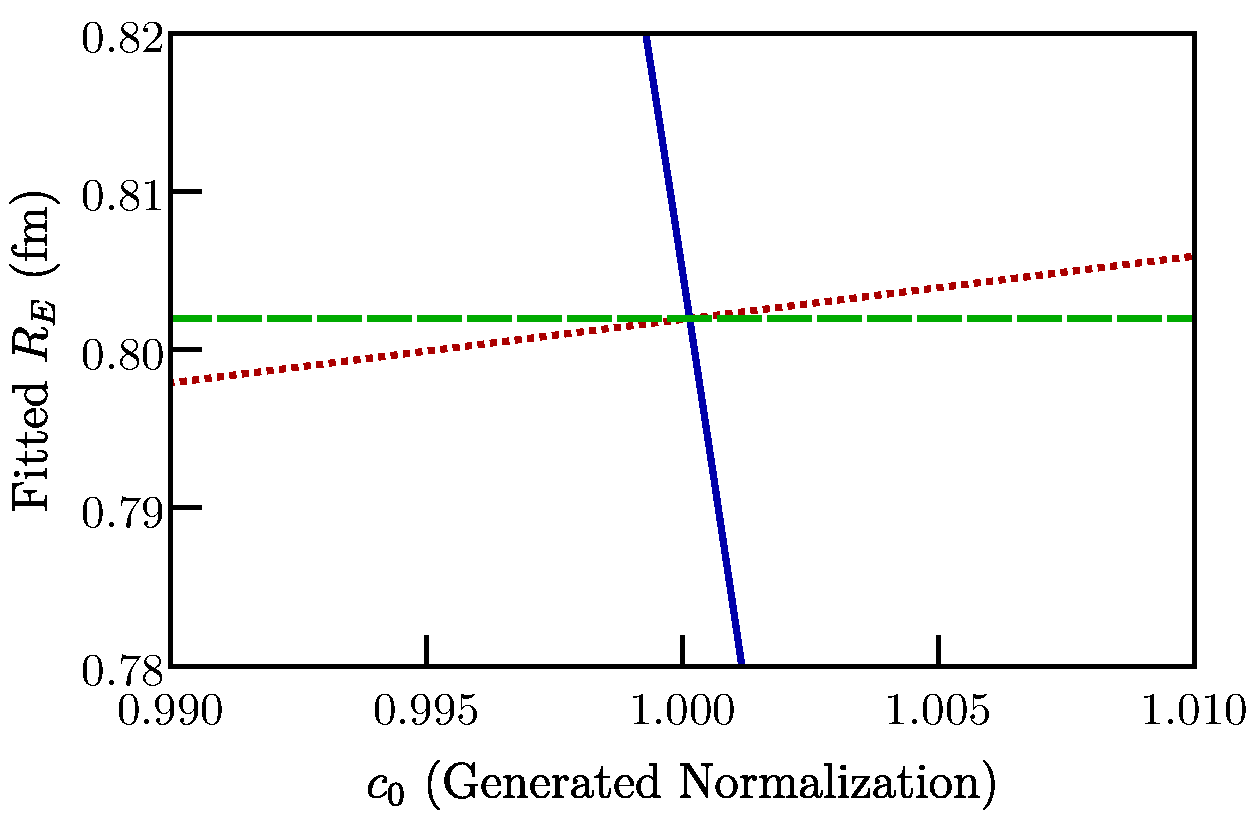
\includegraphics[scale=0.41]{normalization.pdf}
\caption{(Color online). The extracted radius from $1+c_1Q^2$ (solid blue line), $c_0+c_1 Q^2$ (dotted red line) and $c_0(1+c_1 Q^2)$ (dashed green line) as a function of the generated normalization, $c_0$. $c_0(1+c_1 Q^2)$ yields a stable result independent of the generated normalization. The dipole radius (0.811~fm) is not accurately reproduced because of bias in the fit form.}
\label{normalization}
\end{figure}

\subsection{The Role of $\chi^2$}

Fits to experimental data typically rely on the minimization of
\begin{align}
\chi^2 = \sum_i^N \left(\frac{G_E\left(Q_i^2 \right) - f(Q_i^2)}{\sigma_i} \right)^2,
\end{align}
in which $G_E(Q_i^2)\pm \sigma_i$ are the data values and $f(Q_i^2)$ are the parameterized fit values at $Q_i^2$. A good fit is expected to have $\chi^2/\text{dof}~\approx~1$, in which the degrees of freedom (dof) are the number of data points minus the number of free parameters. But $\chi^2/\text{dof}$ can be misleading if experimental uncertainties are under- or over-estimated. Additionally, it is frequently possible to obtain different fits to the same data and still arrive at a satisfactory $\chi^2$. 

This can be demonstrated with the Mainz (2010)~\cite{Mainz2010} data from spectrometer B with $Q^2~<~0.02$~GeV$^2$. We used the $P_{2,0}$ and created functions from 500 evenly spaced constants with $\sqrt{6 c_1} \hbar c~=~R_E$ in [0.750,~0.950]~fm and $c_2$ in [-30.0, 30.0]~GeV$^{-4}$ for a total of $500^2$ parameterizations. We calculated the $\chi^2/$dof for each parameterization. FIG. \ref{heat_plot} shows $\chi^2$/dof plotted as a function of the proton radius and curvature terms in $P_{2,0}$ for a normalization of $c_0 = 1$. The $\chi^2$/dof alone implies a wide range of acceptable radii from $\approx$ 0.84 to 0.90~fm. This $\chi^2$ trench arises when increased quadratic curvature is offset by a larger slope at the origin. 
\begin{figure}[h!]
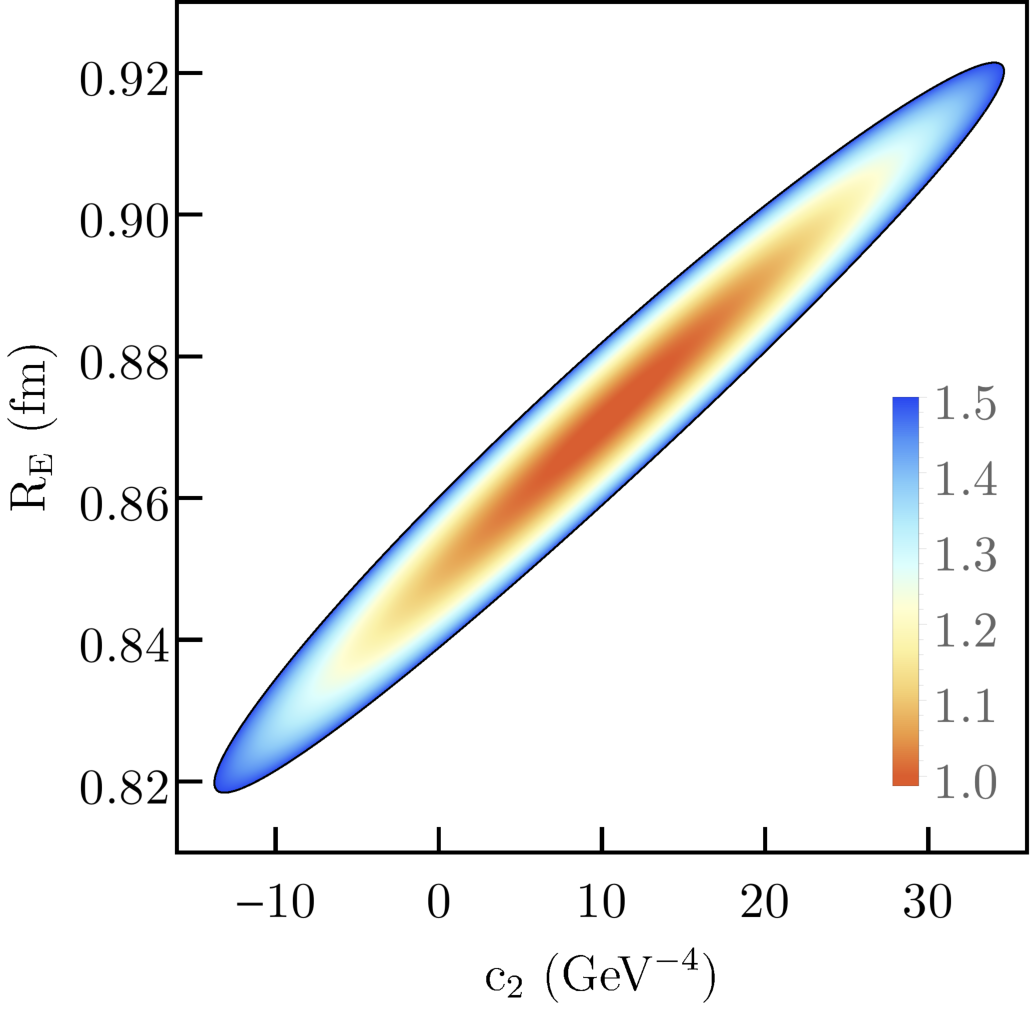
\includegraphics[scale=0.45]{heat_plot_mathematica.pdf}
\caption{(Color online). Two-dimensional $\chi^2/\text{dof}$ surface for the low-$Q^2$ Mainz (2010) data fit to $P_{2,0}$ as a function of the parameters $R_E$ and $c_2$. The $\chi^2$/dof surface indicates a wide range of acceptable radii.}
\label{heat_plot}
\end{figure}

This is demonstrated in another way in FIG. \ref{varied_good_fits}. Three different fits of the $P_{2,0}$ function to the low-$Q^2$ Mainz~(2010) data are pictured. Each fit has a $\chi^2$/dof near unity but their extracted radii vary by more than 0.1~fm. These are visually similar above $Q^2~\approx~0.0075$~GeV$^2$ but differ significantly at lower $Q^2$ where there is no data. These results should be a caution that a good $\chi^2$/dof value alone does not imply a quality radius extraction.  

\begin{figure}[h!]
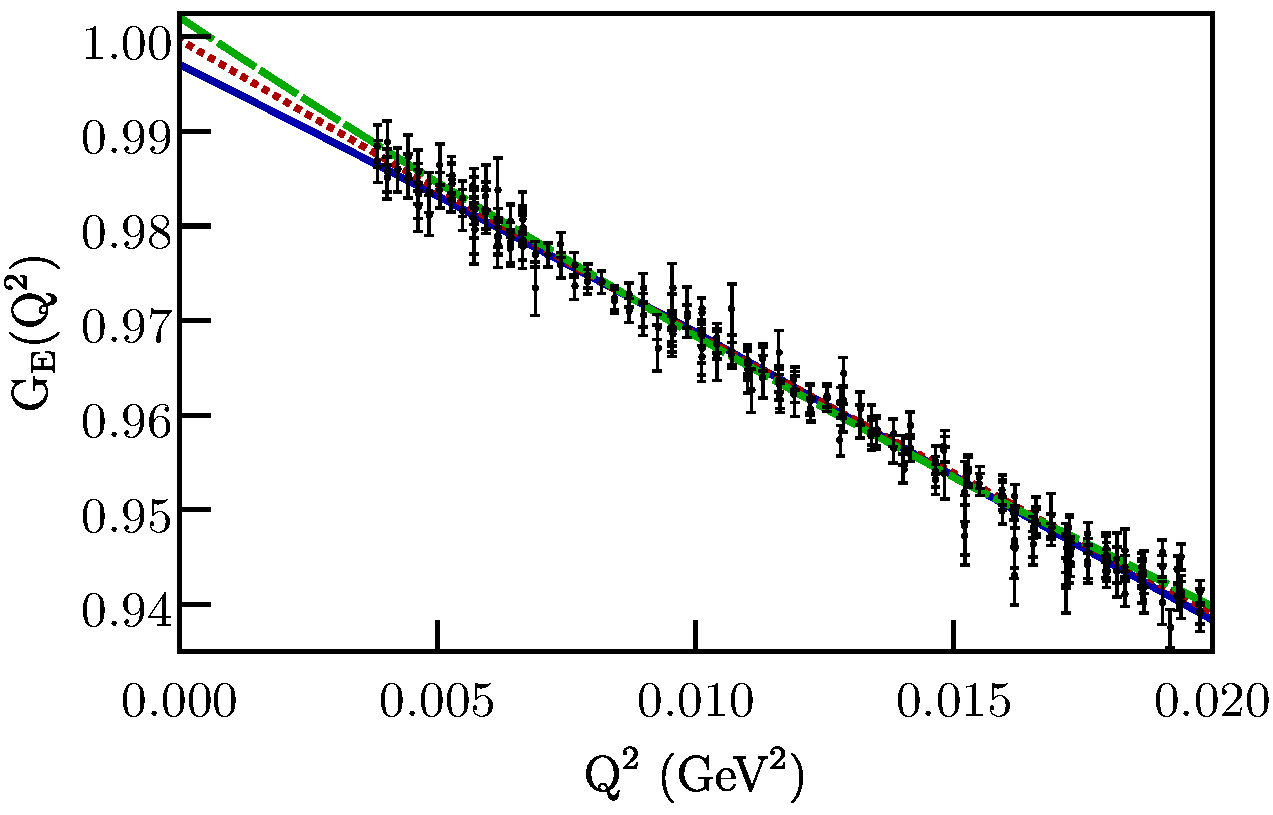
\includegraphics[scale=0.41]{varied_good_fits.pdf}
\caption{(Color online). Three $P_{2,0}$ fits of the Mainz low-$Q^2$ data with low $\chi^2$/dof but extracted radii differing by more than 0.1~fm. The solid blue line has a radius of 0.800~fm and $\chi^2$/dof~=~1.033, the dotted red line has a radius of 0.865~fm and $\chi^2$/dof = 0.986 and the dashed green line has a radius of 0.920~fm with a $\chi^2$/dof = 1.025. Note that the fits are not constrained to $G_E(0)=1$ because of the normalization constant.} 
\label{varied_good_fits}
\end{figure}

Any experimental measurement is just a single instance in a range of possible values governed by statistical variance. To understand the implications of this variance, we generated a data set with 15 points using the $P_{1,0}$ function with 1\% uncertainty on each point. Each point was then shifted by a random value chosen from a Gaussian distribution with $\sigma$ set by the uncertainty on the point. Then the data set was refit using $P_{1,0}$. This process was repeated 10,000 times. The resulting distribution of $\chi^2$ values, as expected, was a $\chi^2$ distribution with $k$ degrees of freedom, given by
\begin{align}
f(x,k) &= \frac{x^{\frac{k}{2}-1}e^{-\frac{x}{2}}}{2^{\frac{k}{2}}\Gamma\left( \frac{k}{2} \right)},
\end{align}
in which $\Gamma$ denotes the Euler-gamma function and $x > 0$.

For a data set with 15 points, fit to $P_{1,0}$, we expected $k=13$. FIG.~\ref{chi2_distros} shows the $\chi^2$ distribution for $k=13$ with the data (blue circles) agreeing well. Despite this agreement for the distribution, it is possible for a single fit to return a $\chi^2$ value much larger or smaller than $\chi^2/\text{dof}~=~1$. A single measured unsatisfactory value for $\chi^2$ from experimental data does not necessarily indicate a poor estimate of a fitted parameter.

\begin{figure}[h!]
	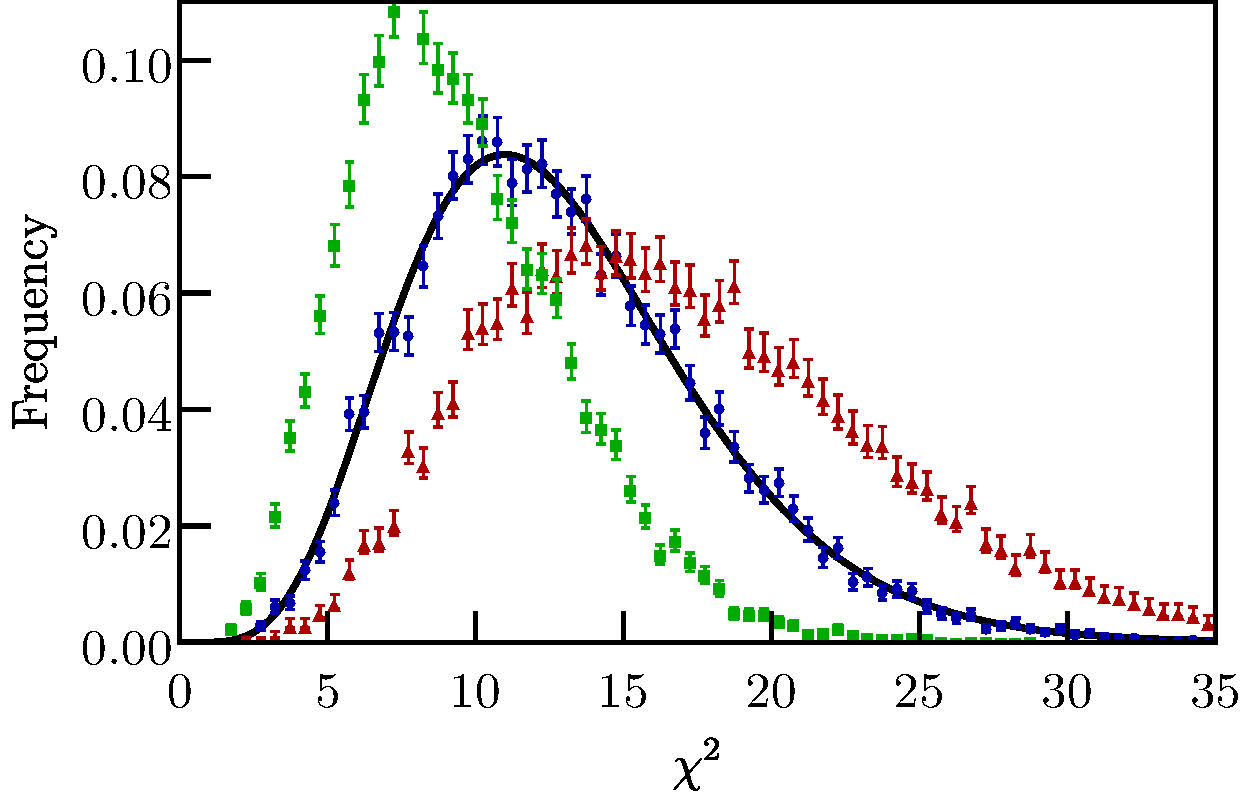
\includegraphics[scale=0.41]{chi2_distros.pdf}
	\caption{(Color online). Histogram of $\chi^2$ values for data created by allowing the data points to fluctuate within their variance by $\sigma$ (blue circles), $1.15 \sigma$ (red triangles) and $0.85 \sigma$ (green squares). The solid black line is the expected $\chi^2$ distribution.}
	\label{chi2_distros}
\end{figure}

Over- or under-estimated point-to-point errors introduce a potential problem. We studied this by repeating the above procedure but instead shifted by a random value chosen from a Gaussian distribution with width equal to $1.15 \sigma$ (red triangles, representing quoted error bars that are too small) and $0.85 \sigma$ (green squares, representing quoted error bars that are too large). The results for these distributions of $\chi^2$ are also pictured in FIG.~\ref{chi2_distros}. If the statistical uncertainties on the data points are not representative of true Gaussian statistics, it may not be accurate to say that a poorly reconstructed $\chi^2$ distribution indicates a bad extraction.

For each fit in this paper we quote the quantity $k'/k$ as an indicator of the statistical reliability of the experimental error estimates on the data points. Here $k$ is the number of degrees of freedom of the fit and $k'$ is the number of degrees of freedom obtained by fitting the distribution of $\chi^2$ values from the 10,000 fits. In Monte Carlo tests we found that the ratio $k'/k$ was always proportional and nearly equal (within 10\%) to $\sigma'/\sigma$, where $\sigma'$ corresponded to a rescaled value of the experimental uncertainties. Consequently if the experimental uncertainties are over-estimated, $k'/k<1$ and if the uncertainties are under-estimated, $k'/k>1$. Although this typically does not change the central values for $R_E$, it does affect the uncertainty quoted for $R_E$. This factor is not included in our uncertainty estimated for $R_E$ from the archival data sets but is listed in the data tables.

\subsection{Fitting Algorithm}
We embarked on a analysis of archival data to better understand the current limitations on nuclear radii extracted from fits of form factor data. Our goal was to create a consistent process that worked to simultaneously minimize both the statistical uncertainty and possible bias stemming from the chosen fit model. For each data set, we took the published data at face value and accepted reported uncertainties as statistically distributed. The fitting procedure was as follows.

We first attempted to estimate the bias of each fit form over the range of possible $Q^2$ upper bounds of the examined data set. This was done by generating pseudodata with the generating functions discussed in Section \ref{models}, over the range of $Q^2$ values present in the examined data set. These pseudodata were then fit with the proposed fit forms from their first point to the $i$th point, and then the $i$th$+1$ point, and so on, until the entire data set had been fit. The value $i$ was the minimum number of data points necessary for each function. The bias was determined to be the rms value of the difference between the input radii in the generating functions and the extracted radii from the fit functions. This value was calculated for each investigated potential fit function and each possible $Q^2$ upper bound. The results of this procedure for the Mainz (1980)~\cite{Mainz1980} data set are pictured in FIG.~\ref{systematic_bias}, which allows us to estimate the bias of each potential fit as a function of the $Q^2$ upper bound. The functions with fewer parameters ($P_{1,0}$ and $P_{0,1}$) produce systematically higher biases than the functions with more parameters ($P_{2,0}$, $P_{0,2}$ and ${CF}_2$).

\begin{figure}[h!]
	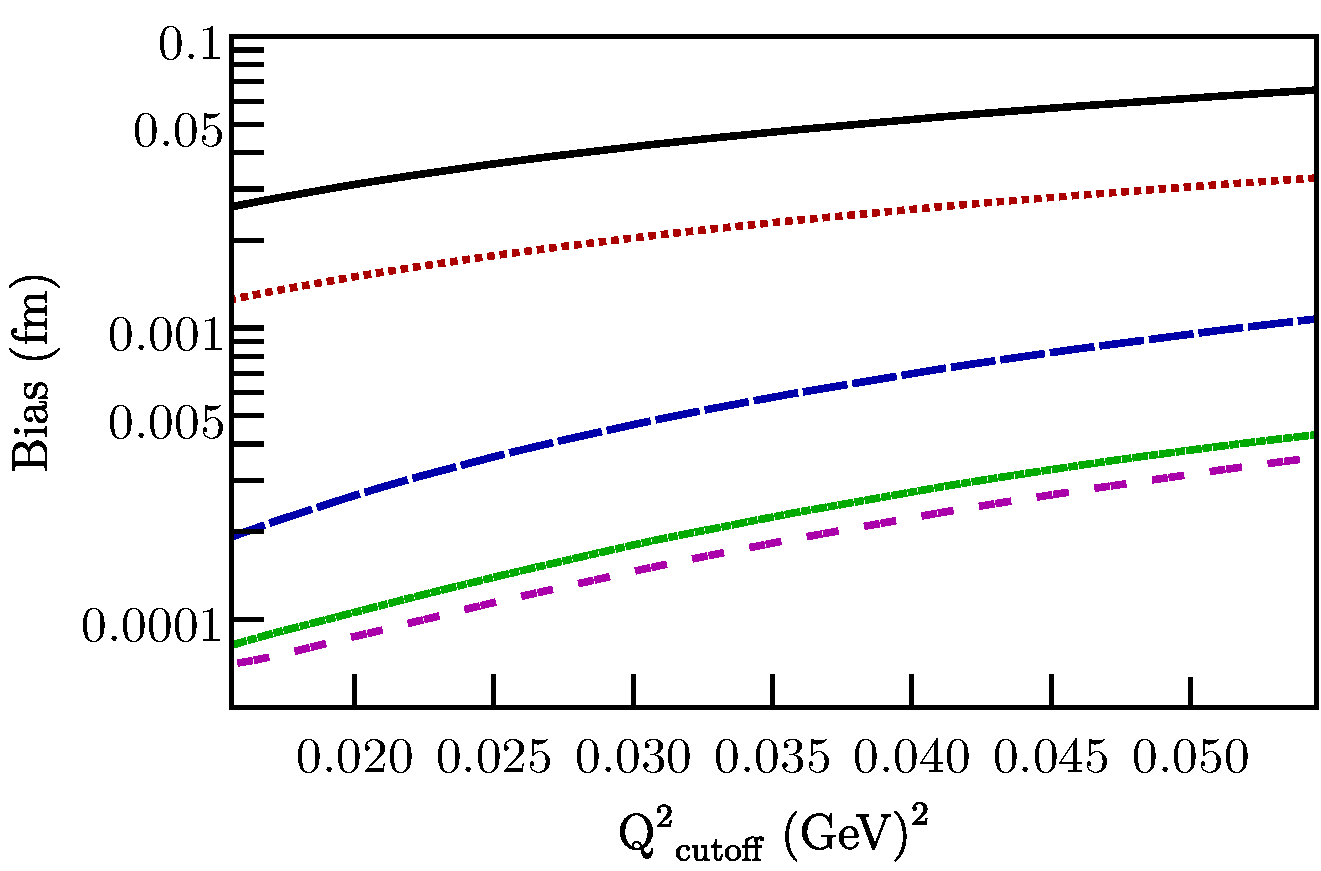
\includegraphics[scale=0.39]{bias_example.pdf}
	\caption{(Color online). The systematic bias of each fit function over the range in possible $Q^2$ upper bounds for the Mainz (1980) data set. The functions with one parameter, $P_{1,0}$ (solid black line) and $P_{0,1}$ (dotted red line), show less flexibility and a corresponding increase in bias than do the functions with two parameters, $P_{2,0}$ (dashed blue line), $P_{0,2}$ (dash-dotted green line) and ${CF}_2$ (double dashed magenta line).}
	\label{systematic_bias}
\end{figure}

We next attempted to constrain the quality of the fit. We fit the data from the lowest $Q^2$ point out to every possible $Q^2$ upper bound, this time using the real archival data sets. The residuals of these fits were then fit to the function $c_1 + c_2 Q^2 + c_3 Q^4$. An example of this for the Mainz~(1980) data set with residuals from the ${CF}_{2}$ function is shown in FIG \ref{residuals_example}. These residuals were shifted by a value randomly chosen from a Gaussian distribution whose width was equal to their uncertainty and refit to the quadratic function. This process was repeated 10,000 times and a quality fit was defined as one that had a statistical uncertainty on each $c_i$ that was within 1$\sigma$ of zero. 

\begin{figure}[h!]
	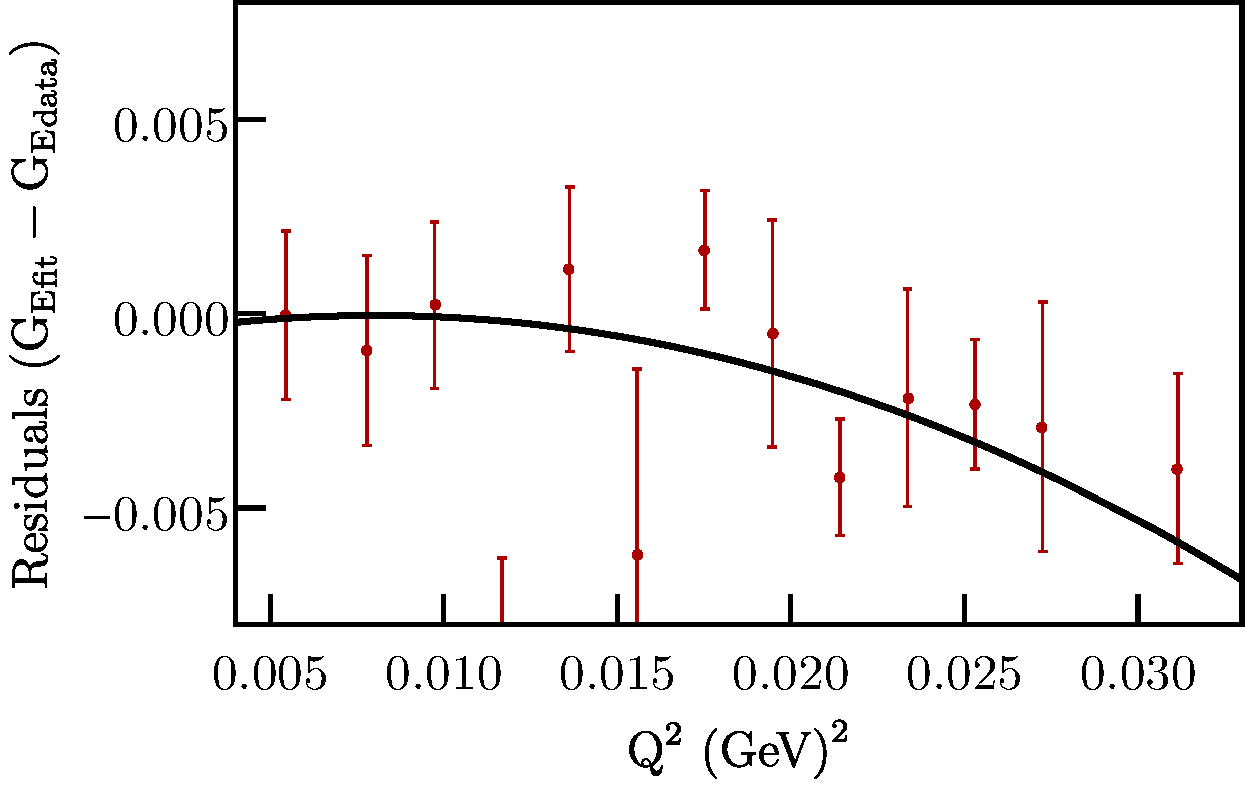
\includegraphics[scale=0.41]{residuals_example.pdf}
	\caption{The residuals of the Mainz (1980) data set fit to the ${CF}_2$. The residuals themselves have been fit to a quadratic function, pictured in black.}
	\label{residuals_example}
\end{figure}

To determine the statistical uncertainty (variance) on the extracted radius, the individual points in the data set were also randomly shifted based on their uncertainty and the data were refit. This process was repeated for each fit function and $Q^2$ upper bound and the statistical uncertainty in each case was taken to be the rms variation of the 10,000 extracted radii. This method is consistent with the standard $\chi^2$ minimization technique: for the full Mainz (1980) data set, the ${CF}_2$ returns a radius with an uncertainty of 0.027~fm for the Gaussian Monte Carlo method and 0.026~fm for the $\chi^2$ method. 

The statistical uncertainty as a function of $Q^2$ upper bound for the Mainz (1980) data set is pictured in FIG. \ref{uncertainty}. More complex functions ($P_{2,0}$, $P_{0,2}$ and ${CF}_2$) generally produce larger variances but smaller biases. The best fit function and $Q^2$ upper bound will minimize the combination of variance and bias. We limited ourselves to fits with variances at least twice as large as the systematic bias. This was done so that the final error was not dominated by bias and because the variance is symmetric about the central value whereas bias is one-sided. 

\begin{figure}[h]
	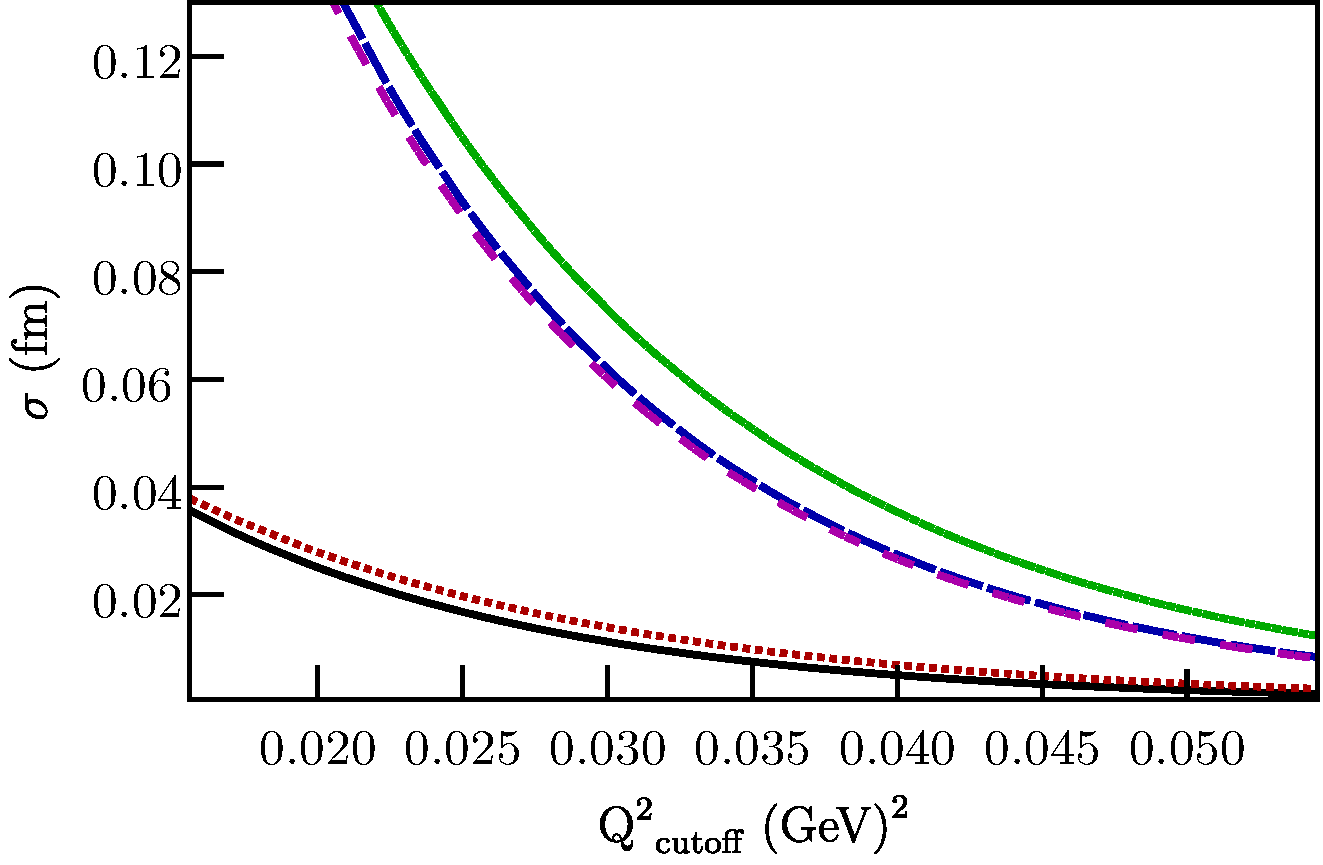
\includegraphics[scale=0.385]{uncertainty_exmample}
	\caption{(Color online). The statistical uncertainty of each fit function over the range in possible $Q^2$ upper bounds for the Mainz (1980) data set. The functions with one parameter, $P_{1,0}$ (solid black line) and $P_{0,1}$ (dotted red line), produce smaller uncertainties than the functions with two parameters, $P_{2,0}$ (dashed blue line), $P_{0,2}$ (dash-dotted green line) and ${CF}_2$ (double dashed magenta line).}
	\label{uncertainty}
\end{figure}

The radius chosen for each data set was extracted using the particular function and $Q^2$ upper bound that a) produced residuals whose parameters were consistent within $1\sigma$ of zero, b) had a statistical uncertainty that was at least twice the systematic bias and c) had the lowest linear sum of the statistical variance and systematic bias of candidates that passed the first two tests. In this way we aimed to ensure a reasonable fit of the data while simultaneously minimizing the bias in the extrapolation and the sum of bias plus variance in the quoted radii.

\section{Historical Data}
\subsection{20th Century Proton Data}

In total we examined 5 early $ep$ scattering data sets. The first, Hand et al. (1963)~\cite{Hand1963} gave a review of scattering data before 1963. We use the published values of $G_E$ below 0.116~GeV$^2$~(3~fm$^{-2}$) for a loose definition of ``low-Q$^2$." These data were comprised of points from 5 different experiments and the $G_E$ values were derived from a Rosenbluth separation of the cross section data for $Q^2 \geq 0.078$~GeV$^2$ and by implicit assumption that $G_M = \mu G_E$ for values with $Q^2 \leq 0.078$~GeV$^2$. The next two data sets were Yerevan (1972)~\cite{Yerevan1972} and Saskatoon (1974)~\cite{Saskatoon1974} whose published $G_E$ values were calculated from a Rosenbluth separation. The fourth data set was Mainz (1975)~\cite{Mainz1975} which included published $G_E$ values derived via Rosenbluth separation from experimental cross section values listed in that work and in \cite{Mainz1974}. The final 20th century $ep$ data set was Mainz (1980)~\cite{Mainz1980} which published values for $G_E$ calculated assuming $G_M = \mu G_E$.

The results of applying our algorithm for each 20th century data set are given in TABLE \ref{proton_table}. The 20th century weighted average radius is 0.856(16)~fm which is in agreement with the muon spectroscopy value, albeit with substantially larger error bars.  FIG. \ref{progression_of_radii} shows the results for each 20th century data set and the weighted average fit compared with the muon spectroscopy and CODATA values. 
\begin{figure}[h!]
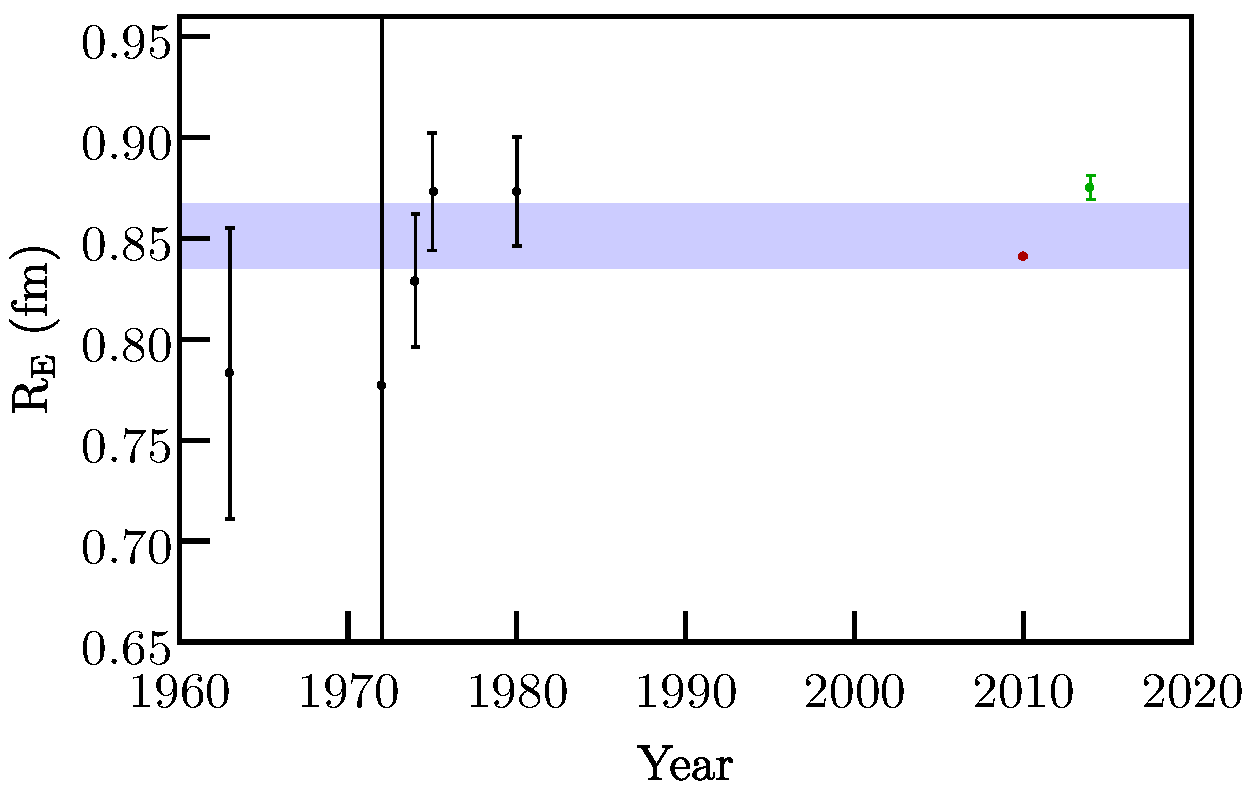
\includegraphics[scale=0.41]{progression_of_radii.pdf}
\caption{(Color online). The proton radii extracted from the 20th century experiments (black), compared to the 2010 muon spectroscopy result, 0.84087(39)~fm (red), and the 2014 CODATA result, 0.875(6)~fm (green). Our 20th century average, 0.856(16)~fm, is shown as a blue band.}
\label{progression_of_radii}
\end{figure}

\subsection{Mainz 2010}

The Mainz 2010 \cite{Mainz2010} data set dominates the low-$Q^2$ landscape. We considered it separately from the 20th century data and examined only the data from spectrometer B (the spectrometer with the lowest $Q^2$~values). This minimized problems arising from normalization adjustments between multiple spectrometers. 

We found the optimal fit for the Mainz (2010) data to be the ${CF}_3$ function with an upper bound of $Q^2~=~0.150$~GeV$^2$ which produced a radius of 0.859(2)~fm. This measurement is in agreement with our 20th century average, 0.856(16)~fm, but sits between the muon spectroscopy and CODATA results. The choice for this $Q^2$ upper bound is demonstrated in FIG. \ref{sum_error}, where the variance plus bias is shown as a function of $Q^2$ upper bound. It is not always the case that increasing the maximum $Q^2$ value will improve the combination of variance and bias.

\begin{figure}[t]
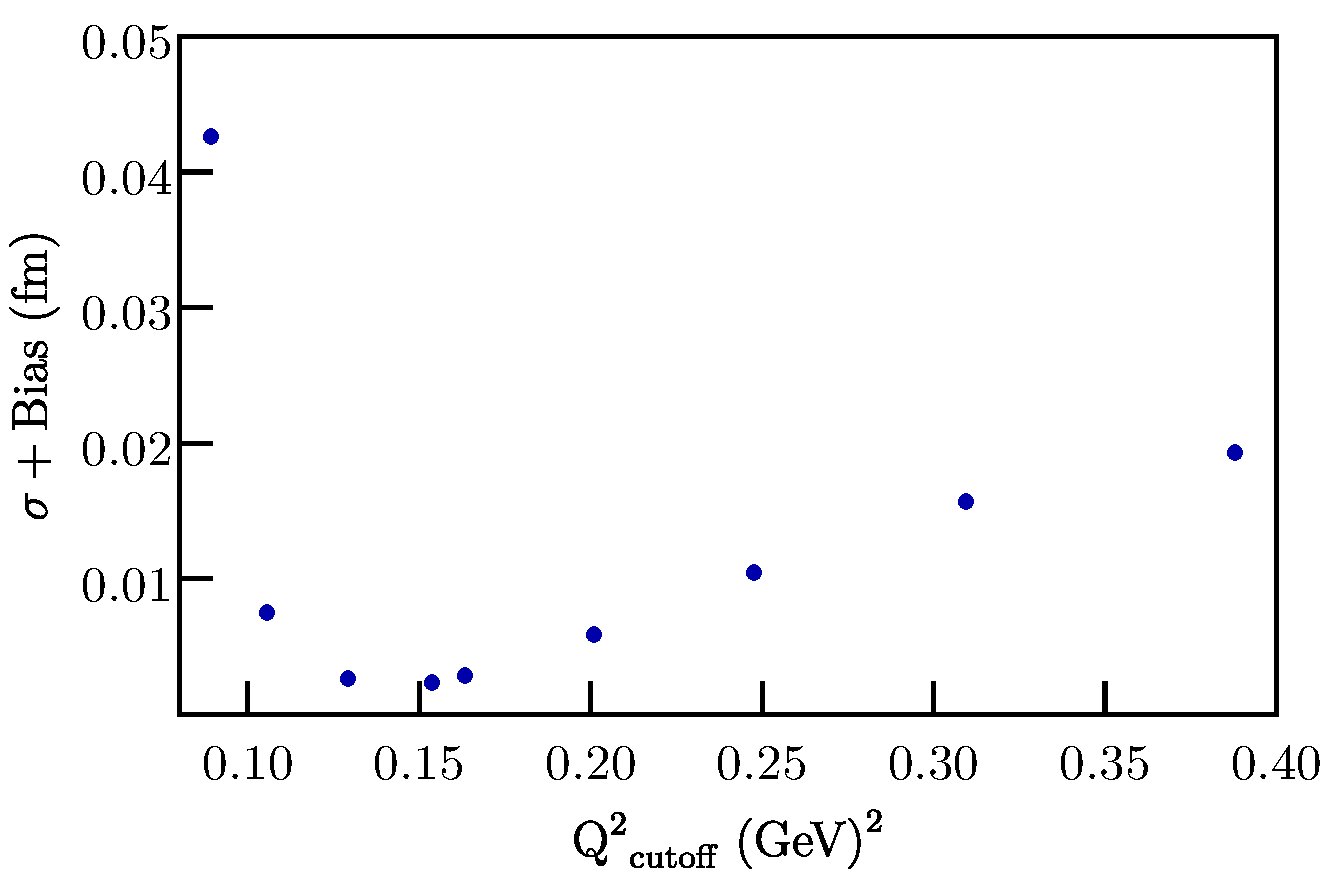
\includegraphics[scale=0.39]{sum_error.pdf}
\caption{(Color online). Total error (variance + bias) for the Mainz (2010) data set fit to the ${CF}_3$ function. There is a minimum around $Q^2 = 0.150$~GeV$^2$ which the algorithm chose for the $Q^2$ upper bound.}
\label{sum_error}
\end{figure}

The results of our fitting algorithm for each $ep$ data set are given in TABLE \ref{proton_table} and each data set along with its corresponding fit is plotted in FIG. \ref{proton_aggregate}. The $CF_2$ is generally preferred below $0.10$~GeV$^2$ because it is the most adaptive function analyzed and thus results in the lowest bias values (see FIG. \ref{systematic_bias}) while not having the largest uncertainties (see FIG. \ref{uncertainty}). 

\begin{figure}[t]
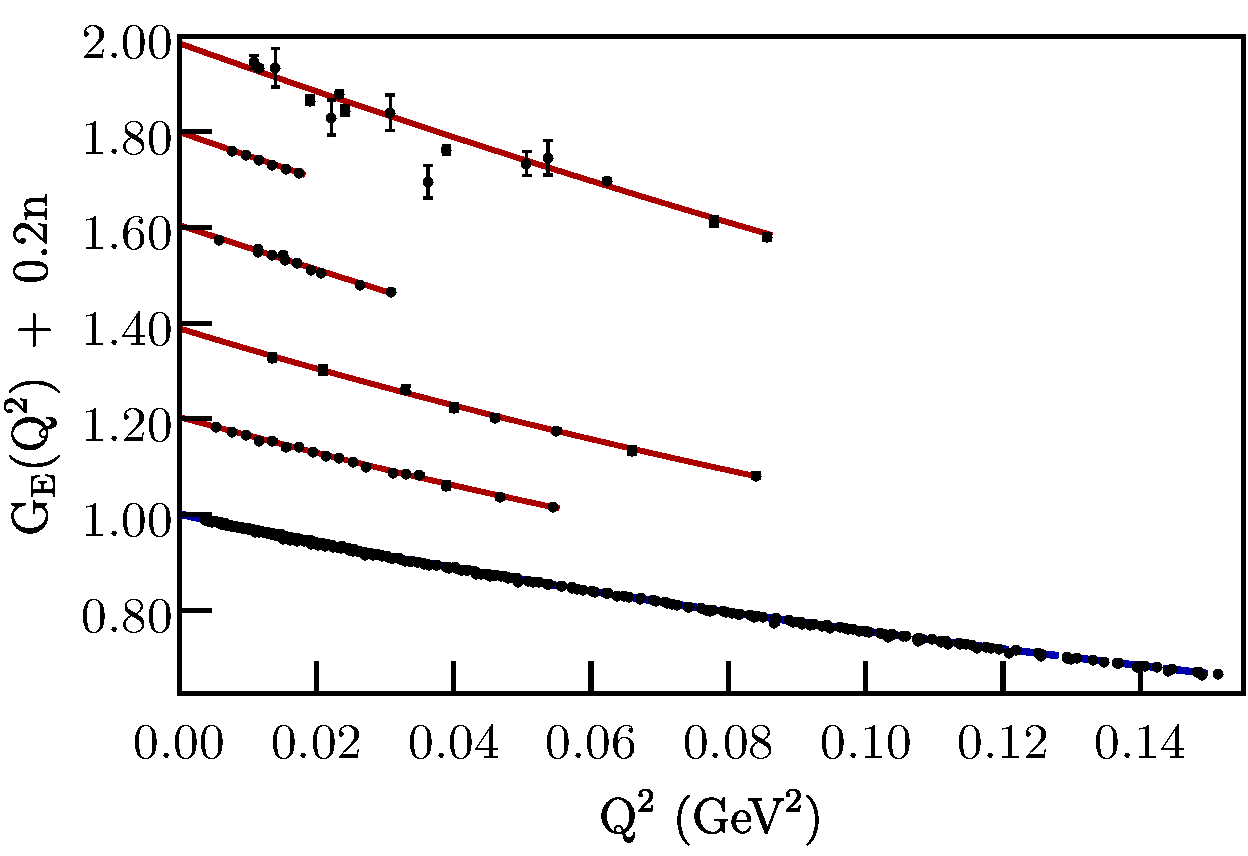
\includegraphics[scale=0.40]{proton_aggregate_plot.pdf}
\caption{(Color online). Proton $ep$ scattering data sets and their corresponding fits in chronological order from top to bottom: Hand et al. (1963), Saskatoon (1974), Mainz (1975), Mainz (1980) and Mainz (2010). The dashed blue line is a ${CF}_3$ fit and the solid red lines are ${CF}_2$ fits. Data sets are shifted vertically for visibility}
\label{proton_aggregate}
\end{figure}

\subsection{Deuteron Scattering}
For the deuteron we focused on fitting $A(Q^2)$ from two low-$Q^2$ data sets: Simon et al.~(1981)~\cite{Simon1980}, which published $A(Q^2)$ values calculated directly from the cross section for $Q^2 \leq 0.04$~GeV$^2$ and via Rosenbluth separation for $Q^2 \geq 0.04$~GeV$^2$ and Platchkov et al.~(1990)~\cite{Platchkov1990} where we used published $A(Q^2)$ values below $Q^2~=~0.116$~GeV$^2$ calculated by subtracting $B(Q^2)$ contributions from the cross section using a fit of existing $B(Q^2)$ measurements.

For the Simon et al.~(1981) data set the ${CF}_4$ fit is favored out to 0.156~GeV$^2$, which yields a radius of 2.104(14)~fm. For the Platchkov et al.~(1990) data set the ${CF}_3$ fit is preferred and the extracted radius is 2.149(78)~fm. The full results for the $ed$ scattering experiments are listed in TABLE \ref{deuteron_table} and each data set, along with its corresponding fit, is plotted in FIG. \ref{deuteron_aggregate}. The combined rms radius for the deuteron is 2.105(14)~fm, which is about 3$\sigma$ below the CODATA value of 2.142(2)~fm and about 2$\sigma$ below the muonic lamb shift measurement of 2.1256(8)~fm.

\begin{figure}[h]
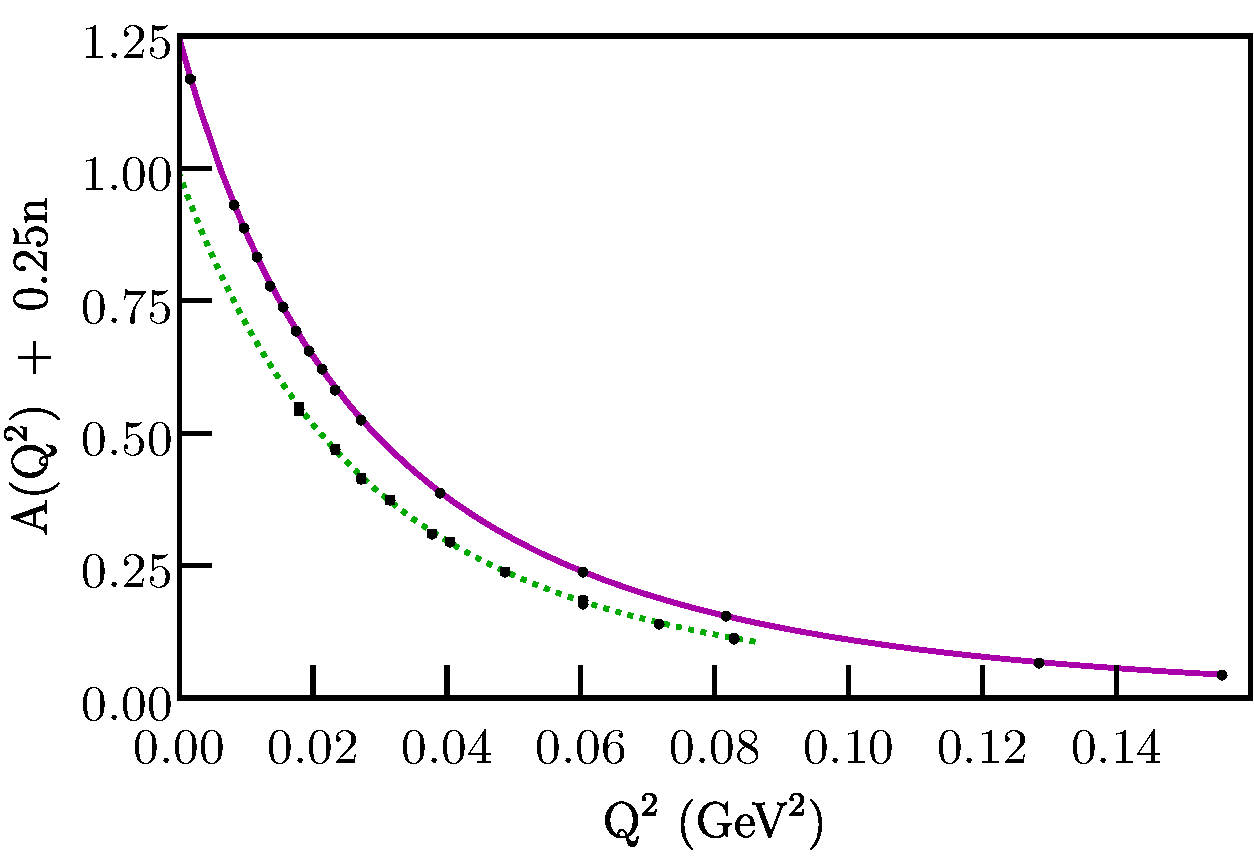
\includegraphics[scale=0.40]{deuteron_aggregate_plot}
\caption{(Color online). Deuteron $ed$ scattering data sets and their corresponding fits. The dashed green line is a ${CF}_3$ fit to the Platchkov et al.~(1990) data set fit and the solid magenta line is a ${CF}_4$ fit to the Simon et al.~(1981) data set. Data sets are shifted vertically for visibility. }
\label{deuteron_aggregate}
\end{figure}

\section{Future Experiments}
The statistical precision of the Mainz (2010) data set dwarfs the combined precision of the rest of the $ep$ scattering data. Additional data sets with at least comparable statistics are necessary to firmly establish the proton radius from elastic-scattering. Several upcoming $ep$ scattering experiments will shed further light on the proton radius problem. Based on our work, we suggest methods for fitting these upcoming data and present possible results based on simulated data.

\subsection{PRad}
The PRad~\cite{PRad} experiment performed a magnetic-spectrometer-free elastic-scattering experiment for the first time. Data were collected using a windowless gas jet target and the analysis is currently ongoing. We analyzed a simulated data set of the PRad experiment and found the optimal fit to be the ${CF}_2$ function out to $Q^2~=~0.082~$GeV$^2$. The resulting statistical uncertainty will be about about 0.009~fm. Our choice of fit function is consistent with~\cite{PRad_data}.

\subsection{A2}
A proposal being developed for the A2 Hall at MAMI, Mainz intends to measure the recoiling protons in elastic scattering from 0.001 $\leq Q^2 \leq$ 0.04~GeV$^2$ using an active-target time projection chamber. The intention is to run for 45 days of beam time at 0.5~GeV with estimates of obtaining about 75 million events. We found the optimal fit to be the ${CF}_{2}$ out to $Q^2$ = 0.038~GeV$^2$ with a predicted uncertainty of 0.005~fm. 

\begin{widetext}\begin{center}
\begin{table}
		\begin{tabular}{|c |c| c| c| c| c| c| c| c| c| c| c|} 
			\hline
			Data Set & $R_E$ (fm) & Bias~(fm) & $Q^2_\text{min}$ (GeV$^2$) & $Q^2_\text{cutoff}$ (GeV$^2$) & $F(Q^2)$  & $k'/k$ \\ 
			\hline
			Hand et al.  (1963) & 0.783(72) & 0.012 & 0.012 & 0.116 & ${CF}_{2}$  & 1.911 \\
			\hline
			Yerevan (1972) & 0.777(191) & 0.001 & 0.008  & 0.019 &${CF}_2$ & 0.980 \\
			\hline
			Sasktoon (1974) & 0.829(33) & 0.002 & 0.006 & 0.031 & ${CF}_2$ & 1.661 \\ 
			\hline
			Mainz (1975) & 0.873(29) & 0.013 & 0.014 & 0.123 & ${CF}_2$ & 0.617 \\
			\hline
			Mainz (1980) &0.873(27) & 0.003 & 0.005 & 0.055 & ${CF}_2$ & 1.540  \\
			\hline
			Mainz (2010) &0.859(2) & $3.21 \times 10^{-4}$ & 0.004 & 0.150 & ${CF}_3$ &  2.154 \\			
			\hline
		\end{tabular}
		\caption{The results of our fitting algorithm for the examined $ep$ scattering data sets.}
		\label{proton_table}
	\end{table}
\begin{table}
	\begin{tabular}{|c |c| c| c| c| c| c| c| c| c| c| c|} 
		\hline
		Data Set & $R_E$ (fm) & Bias~(fm) &  $Q^2_\text{min}$ (GeV$^2$) & $Q^2_\text{cutoff}$ (GeV$^2$)  & $F(Q^2)$   & $k'/k$ \\ 
		\hline
		Simon (1981) & 2.104(14) & 0.002 & 0.002 & 0.156 & ${CF}_4$  & 1.517 \\
		\hline
		Platchkov (1990) & 2.149(78) & 0.001 & 0.018  & 0.083 & ${CF}_3$ & 0.813 \\		
		\hline
	\end{tabular} 
	\caption{The results of our fitting algorithm for the examined $ed$ scattering data sets.}
	\label{deuteron_table}
\end{table}
		\begin{table}[h!]
			\begin{tabular}{|c |c| c| c| c| c| c| c| c| c| c| c|} 
				\hline
				Data Set & Precision (fm) & Bias~(fm) &  $Q^2_\text{min}$ (GeV$^2$) & $Q^2_\text{cutoff}$ (GeV$^2$)  & $F(Q^2)$  \\ 
				\hline
				PRAD & 0.009 & 0.005 & $3.08\times 10^{-4}$ & 0.082 & ${CF}_2$  \\
				\hline
				A2 & 0.005 & 0.002 & 0.001  & 0.038 &  ${CF}_{2}$ \\		
				\hline
			\end{tabular} 
			\caption{The predictions of our fitting algorithm for upcoming $ep$ scattering experiments.}
			\label{future_experiments_table}
\end{table}\end{center}\end{widetext}

\section{Conclusions}

Using a consistent and comprehensive fitting approach we have arrived at a proton radius measured from $ep$ scattering in the 20th century of $0.856(16)$~fm and a value of $0.859(2)$~fm for the Mainz (2010) experiment. These are smaller than the CODATA value but larger than the muonic hydrogen Lamb shift values. We found a deuteron radius from $ed$ scattering of 2.105(14)~fm which is much smaller than both the CODATA and muonic deuterium Lamb shift values. We stress that systematic uncertainties have not been estimated in this analysis. Systematic errors in the archival data sets could be large enough to account for the discrepancy with muonic lamb shifts. 

Clearly, the current elastic scattering measurements are insufficiently accurate to resolve the linear-quadratic ambiguity at low~$Q^2$ in order to determine $R_E$. Precise new experiments that extend to lower~$Q^2$ are needed and the upcoming PRad and A2 efforts should make valuable contributions toward resolving the proton radius problem. Additionally, upcoming results from a Mainz A1 deuteron scattering experiment should eclipse previous electron scattering studies of the deuteron radius.

\begin{acknowledgments}
We thank the Department of Energy for support under grant DE-FG02-96ER41003. We also thank Carl Carlson and Douglas Higinbotham for useful discussions.
\end{acknowledgments}

\begin{thebibliography}{99}

%%\cite{Carlson:2015jba}
%\bibitem{Carlson:2015jba} 
%  C.~E.~Carlson,
%  %``The Proton Radius Puzzle,''
%  Prog.\ Part.\ Nucl.\ Phys.\  {\bf 82}, 59 (2015)
%  doi:10.1016/j.ppnp.2015.01.002
%  [arXiv:1502.05314 [hep-ph]].
%  %%CITATION = doi:10.1016/j.ppnp.2015.01.002;%%
%  %77 citations counted in INSPIRE as of 17 Aug 2017
  
    \bibitem{Hand1963}
  L. N. Hand, D. G. Miller and Richard Wilson.
  % ``Electric and Magnetic Form Factors of the Nucleon.''
  Review of Modern Physics, {\bf 35}, no 2, pp. 335-349 (1963).
  %%CITATION = 10.1103/RevModPhys.35.335 %%
  
  \bibitem{Yerevan1972}
  Yu. K. Akimov, et al.
  %``Electron Scattering by Protons at Small Angles''
  Soviet Physics JEPT, {\bf 35}, no 4. (1972).
  
  \bibitem{Saskatoon1974}
  J. J. Murphy, II, Y. M. Shin and D. M. Skopik.
  % ``Proton form factors from 0.15 to 0.79 fm$^{-2}$.''
  Phys.\ Rev.\ C {\bf 9}, no 6, (1974).
  
  \bibitem{Mainz1975}
  F Borkowski, G. G. Simon, V. H. Walhter and R. D. Wendling.
  %``Electromagnetic form factors of the proton at low four-momentum transfer.''
  Nuc.\ Phys.\ {\bf B93}, Issue 3, pp 461-478 (1975).
  
    \bibitem{Mainz1974}
    F Borkowski, P. Peuser, G. G. Simon, V. H. Walhter and R. D. Wendling.
   %``Electromagnetic form factors of the proton at low four-momentum transfer.''
   Nuc.\ Phys.\ {\bf A222}, pp 269 - 275 (1974)
  
  \bibitem{Mainz1980}
  G. G. Simon, Ch. Schmitt, F. Borkowski and V. H. Walhter.
  %``Absolute electron-proton cross sections at low momentum transfer measured with a high pressure gas target system.''
  Nuc.\ Phys.\ {\bf A333}, pp. 381-391, (1980).
  
  \bibitem{Mainz2010}
  J. C. Bernauer et al. [A1 Collaboration], Phys. Rev. Lett. 105
  (2010) 242001. [arXiv:1007.5076 [nucl-ex]].
 
  \bibitem{hyd_lamb1}
  M. G. Boshier et al. Phys. Rev. A {\bf40}, 6169 (1989).
  
  \bibitem{hyd_lamb2}
  M. Weitz et al. Phys. Rev. Lett, {\bf72}, 328 (1994).
  
  \bibitem{hyd_lamb3}
  D. J. Berkeland, E. A. Hinds and M. G. Boshier. Phys. Rev. Lett, {\bf75}, 2470 (1995).
  
  \bibitem{hyd_lamb4}
  S. Bourzeix, B. de Beauvoir, F. Nez, M. D. Plimmer, F. de Tomasi, L. Julien, F. Biraben, and D. N. Stacey.
  %``High Resolution Spectroscopy of the Hydrogen Atom: Determination of the 1S Lamb Shift''
  Phys. Rev. Lett. {\bf76}, Number 3, (1996)
  
    \bibitem{hyd_lamb5}
  Th. Udem, A Huber, B. Gross, J. Reichert, M. Prevedelli, M. Weitz and T. W. H\"{a}nsch.
  %``Phase-Coherent Measurement of the Hydrogen 1S-2S Transition Frequency with an Optical Frequency Interval Divider Chain''
  Phys. Rev. Lett. {\bf79}, Number 14, (1997).
  
 
  
  \bibitem{Pohl2010}
   R. Pohl \emph{et al.}, Nature {\bf 466} (2010) 213.
   
   \bibitem{Antognini2013}
   A. Antognini, F. Nez, K. Schuhmann, F. D. Amaro, F. Biraben, J. M. R. Cardoso,
	D. S. Covita and A. Dax et al., Science {\bf 339}, 417 (2013).
	
	  \bibitem{CODATA}
  P. J. Mohr, B. N. Taylor, and D. B. Newell, Rev. Mod. Phys. {\bf 84}, 1527 (2012), 1203.5425.
		
	\bibitem{smallRadii1}
	 I. T. Lorenz and U.-G. Meiner, Phys. Lett. B737, 57 (2014), arXiv:1406.2962 [hep-ph].
	 
	 \bibitem{smallRadii2}
	 K. Griffioen, C. Carlson, and S. Maddox, Phys. Rev. C93, 065207 (2016), arXiv:1509.06676 [nucl-ex].
	 
	 \bibitem{smallRadii3}
	 D. W. Higinbotham, A. A. Kabir, V. Lin, D. Meekins, B. Norum, and B. Sawatzky, Phys. Rev. C93, 055207 (2016),
arXiv:1510.01293 [nucl-ex].

	\bibitem{smallRadii4}
	 M. Horbatsch and E. A. Hessels, Phys. Rev. C93, 015204 (2016), arXiv:1509.05644 [nucl-ex].
	 
	 \bibitem{smallRadii5}
	 M. Horbatsch, E. A. Hessels, and A. Pineda, Phys. Rev. C95, 035203 (2017), arXiv:1610.09760 [nucl-th].
	 
	 \bibitem{largeRadii1}
	  J. Arrington and I. Sick, J. Phys. Chem. Ref. Data 44, 031204 (2015), arXiv:1505.02680 [nucl-ex].
	  
	  \bibitem{largeRadii2}
	  G. Lee, J. R. Arrington, and R. J. Hill, Phys. Rev. D92, 013013 (2015), arXiv:1505.01489 [hep-ph].
	  
	  \bibitem{largeRadii3}
	  D. Borisyuk, Nucl. Phys. A843, 59 (2010), arXiv:0911.4091 [hep-ph].
	  
	  \bibitem{largeRadii4}
	  K. M. Graczyk and C. Juszczak, Phys. Rev. C90, 054334 (2014), arXiv:1408.0150 [hep-ph].
	  
	  \bibitem{largeRadii5}
	  J. C. Bernauer et al. (A1), Phys. Rev. C90, 015206 (2014), arXiv:1307.6227 [nucl-ex].
	 
	 	  \bibitem{Simon1980}
  G. G. Simon, Ch. Schmitt and V. H. Walhter. Nuc.\ Phys.\ {\bf A364}, pp. 285-296, (1981).
  
  \bibitem{Platchkov1990}
  S. Platchkov, A Amroun, S. Anuffret, \emph{et al}. Nuc.\ Phys.\ {\bf A510}, pp. 740-758, (1990).


	
	%\cite{Pohl:2016glp}
	\bibitem{Pohl:2016glp} 
	R.~Pohl {\it et al.},
	%``Deuteron charge radius and Rydberg constant from spectroscopy data in atomic deuterium,''
	Metrologia {\bf 54}, L1 (2017)
	doi:10.1088/1681-7575/aa4e59
	[arXiv:1607.03165 [physics.atom-ph]].
	%%CITATION = doi:10.1088/1681-7575/aa4e59;%%
	%5 citations counted in INSPIRE as of 26 Jun 2017

	 
	 	\bibitem{Mohr}
	P. J. Mohr and B. N. Taylor, Phys.\ Rev.\ Lett. {\bf 72} (200) 351.
	
	\bibitem{Ericson}
	T. E. O. Ericson and M. Rosa-Clot, Nucl. Phys. {\bf A405} (1983) 497.
	
		    %\cite{Abbott:2000ak}
  \bibitem{Abbott:2000ak} 
  D.~Abbott {\it et al.} [JLAB t20 Collaboration],
  %``Phenomenology of the deuteron electromagnetic form-factors,''
  Eur.\ Phys.\ J.\ A {\bf 7}, 421 (2000)
  doi:10.1007/PL00013629
  [nucl-ex/0002003].
  %%CITATION = doi:10.1007/PL00013629;%%
  %90 citations counted in INSPIRE as of 26 Jun 2017
 
  
  
  \bibitem{PRad}
  A. Gasparian. ``The PRad experiment and the proton radius puzzle.'' EPJ Web of Conferences, Vol. 73, (2014).

\bibitem{PRad_data}
  X.~Yan {\it et al.},
  %``Robust extraction of proton charge radius from electron-proton scattering data,''
  arXiv:1803.01629 [nucl-ex].
  %%CITATION = ARXIV:1803.01629;%%

\end{thebibliography}

\end{document}
